%===================================== CHAP 2 =================================
\cleardoublepage

\chapter{Theory}

To understand what sets this system apart from other standard search- and filter mechanics, it is important to understand how CBR works. This chapter elaborates on how CBR works, what recommendation systems are, and what MyCBR is; the tool that was used to implement CBR in Utsida.


\section{Case-based Reasoning}
Case-Based Reasoning (CBR) is a methodology in AI for solving problems, and is essentially based on experience. This experience can be used to solve a large range of problems, including complex combinatorial problems, or yield solutions where uncertainty is involved. \cite{richter2013case} Implied by the name, CBR can be broken down into two main concepts; \textit{cases} and \textit{reasoning}.

\begin{enumerate}
    \item Case: An experience of a solved problem, usually represented as a feature vector (see section \ref{sec:feature_vectors}). A case consists of two parts: a problem description and a solution to the problem. A Case-Based Reasoning System (CBRS) stores all of its cases in a \textit{Case Base}.
    \item Reasoning: The approach of drawing conclusions using cases, given a problem to be solved.
\end{enumerate}

Reasoning in CBR differs from other kinds of reasoning because it does not lead from true assumptions to true conclusions. This means that for two cases with identical problem descriptions, the solution to one of them might not be the solution for the other. The recorded experience in the first case may not be exactly similar to the other case. To be reused, it only has to be \enquote{similar}.

\subsection{Feature Vectors}\label{sec:feature_vectors}
A case is usually represented as a feature vector, consisting of a few to many pairs of attributes and their values. A common example is the diagnosis of a sick patient, where a collection of symptoms and weather the patient has them is the problem description, and the final diagnoses is the solution to the case, as illustrated by table \ref{tab:example_case}


\begin{table}[H]
\centering
\small
\caption{Classic case representation with attribute-value pairs for the problem description and the solution.}
\label{tab:example_case}
\begin{tabulary}{\textwidth}{|L|L|}
\hline
\rowcolor[HTML]{C0C0C0} 
Attribute           & Value     \\ \hline
Nausea              & Yes       \\ \hline
Fever               & Yes       \\ \hline
Malaise             & Dizzy     \\ \hline
Blood pressure      & Normal    \\ \hline
Vision changes      & No        \\ \hline
Shortness of breath & No        \\ \hline
Diagnosis           & Influenza \\ \hline
\end{tabulary}
\end{table}

\subsection{The CBR-Cycle}\label{sec:cbr-cycle}

Aamodt & Plaza\cite{aamodt1994case} defined a model which explain the problem solving cycle in CBR (figure \ref{fig:cbr_cycle}). The cycle defines four distinct processes which a case goes through:

\begin{description}
\item [Retrieve:] The most similar case is retrieved from the system's case base, so that it can be compared to a new case.
\item [Reuse:] The solution to the retrieved case is applied to the new case.
\item [Revise:] Confirms that the proposed solution solves the new case, or if its not applicable.
\item [Retain:] Retains the new case with the given solution in the case base for future usage.
\end{description}

\begin{figure}[H]
    \centering
    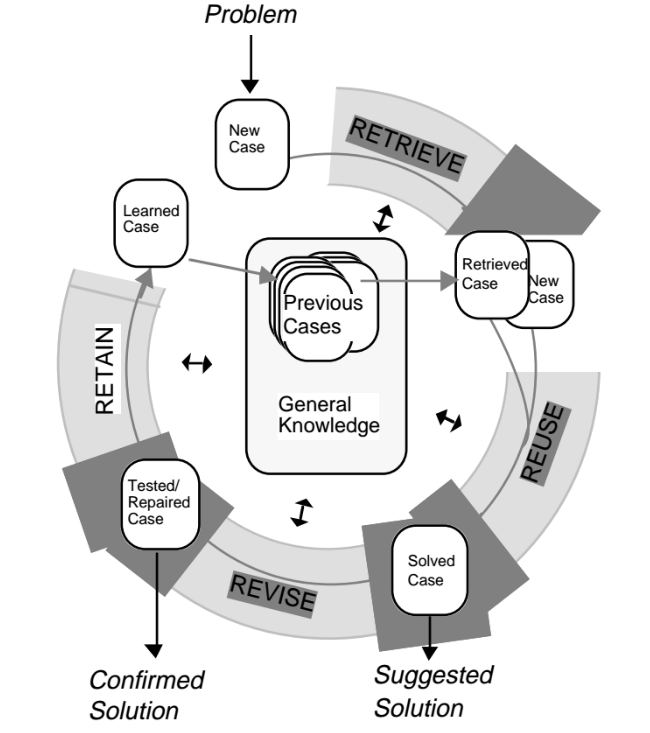
\includegraphics[width=0.6\textwidth]{fig/cbr_cycle.png}
    \caption{The CBR Cycle}
    \label{fig:cbr_cycle}
\end{figure}

\subsection{Similarity Measures}
The degree of similarity between a set of input variables, and a case stored in the case-base is calculated and represented as a \emph{Similarity Measure} (SM). Naturally, a CBRS returns the case or cases with the highest SM. How the SM is calculated is different for each configuration, and must be tailored to each specific system. Typically, each attribute in a case has its own function for calculating the similarity to the identical input-attribute. The most suitable function depends on the attribute's type. For example will a typical function for an integer or float be the polynomial width from the input value, at a given step, while for a string symbol, it can be the the similarity by using approximate string matching. 

Each attribute is given a weight, which decides which attributes are most important, and finally all weights are typically joined by using the \emph{Euclidian Distance}, or \emph{Weighted Sum} methods.

\section{Tools and frameworks}

Due to the increasing popularity of CBR applications\cite{kolodner2014case}, many tools have been developed to model and implement a CBRS. These tools makes it easier to test ideas and develop prototypes without having to start from scratch. This section will introduce some of the different approaches to tool-kits and the reasoning for the selected tool of this research project. 

\subsection{JColibri}
JColibri is an object-oriented framework in Java for building CBR systems, which follows the task/method division paradigm.\cite{bello2004jcolibri} The notion of this paradigm is that each task in a CBR-cycle described in section \ref{sec:cbr-cycle} involves several specific sub-tasks, and instead of using one method on each task, they are decomposed and structured in a way so that different methods can be applied to the different sub-tasks. All though this framework is flexible in terms of the problem domain it will be used for, and can be used for any number of the steps in the CBR-cycle, it required a substantial amount of knowledge for the developers because they have to use appropriate methods for different tasks, go more in depth than other frameworks.


\subsection{CBR-Works}
CBR-Works is a shell for Case-Based application building, which covers the whole CBR-cycle from retrieving to revising, and supports modelling the structure of cases, and maintaining the case base.\cite{schulz1999cbr} It comes with a interface which can be used to build a new Case-Based application from existing data. The framework can be used to construct complex concepts, and includes a rather unique element when modelling the cases; rules. These can be used to set constraints to the concepts for their adaption and completion process. All though this framework is a candidate for this research, it was desired to find a framework which is easier to dive into.

\subsection{MyCBR}
MyCBR is a tool for rapid prototyping of CBR systems with focus on the retrieval step of the CBR cycle.\cite{MyCBR}. Its developed and maintained as a joint project between the German Research Center for Artificial Intelligence (DFKI) and the School of Technology and Computing at the University of West London (UWL)\cite{Stahl2008}. MyCBR was chosen as the designated tool to model the CBRS, because it includes all the necessary functionality, as well as requireing a minimum of domain knowledge, and knowledge about the tool itself. Furthermore, using this tool would make getting help and support easier, considering NTNU has an employee whom is a contributor to the project. MyCBR was used extensively throughout the project to assist with both prototyping and modelling the CBRS. The MyCBR project is first and foremost a Java Software Development Kit (SDK), but also includes a pre-built GUI called the MyCBR Workbench. 

\subsubsection{MyCBR SDK}
The MyCBR SDK provides an access point for implementing the functionality of MyCBR in a custom application. The SDK is written in the JAVA programming language and has executable programs for macOS, Windows and Linux\cite{MyCBR}. 

The current version of the SDK and MyCBR focuses and has implemented only the similarity based retrieval step of the CBR cycle. The myCBR developers reason that this it is due to most applications having the first part as its core functionality\cite{Stahl2008}.  

A recent update extended the SDK to include a REST API that enables cross server communication and requests to MyCBR. This allows an external server to use many of the implemented functionalities in MyCBR SDK as Querying and retrieval.

\subsubsection{MyCBR Workbench}

The myCBR workbench provides a graphical user interface (GUI) of the features in the SDK. This allows easier prototyping and usage for users without the need to have large knowledge of the SDK's inner functions\cite{bach2014knowledge}. 

To be able to quickly import data and cases, the workbench supports importing pre-defined cases with the CSV file format. All the required cases can therefore be gathered and refined before being tested in the workbench. The workbench also supports a set of similarity functions that are easy to model such as Taxonomy and integer functions. The workbench visualises these similarity measures with graphs and tables.

\begin{figure}[H]
    \centering
    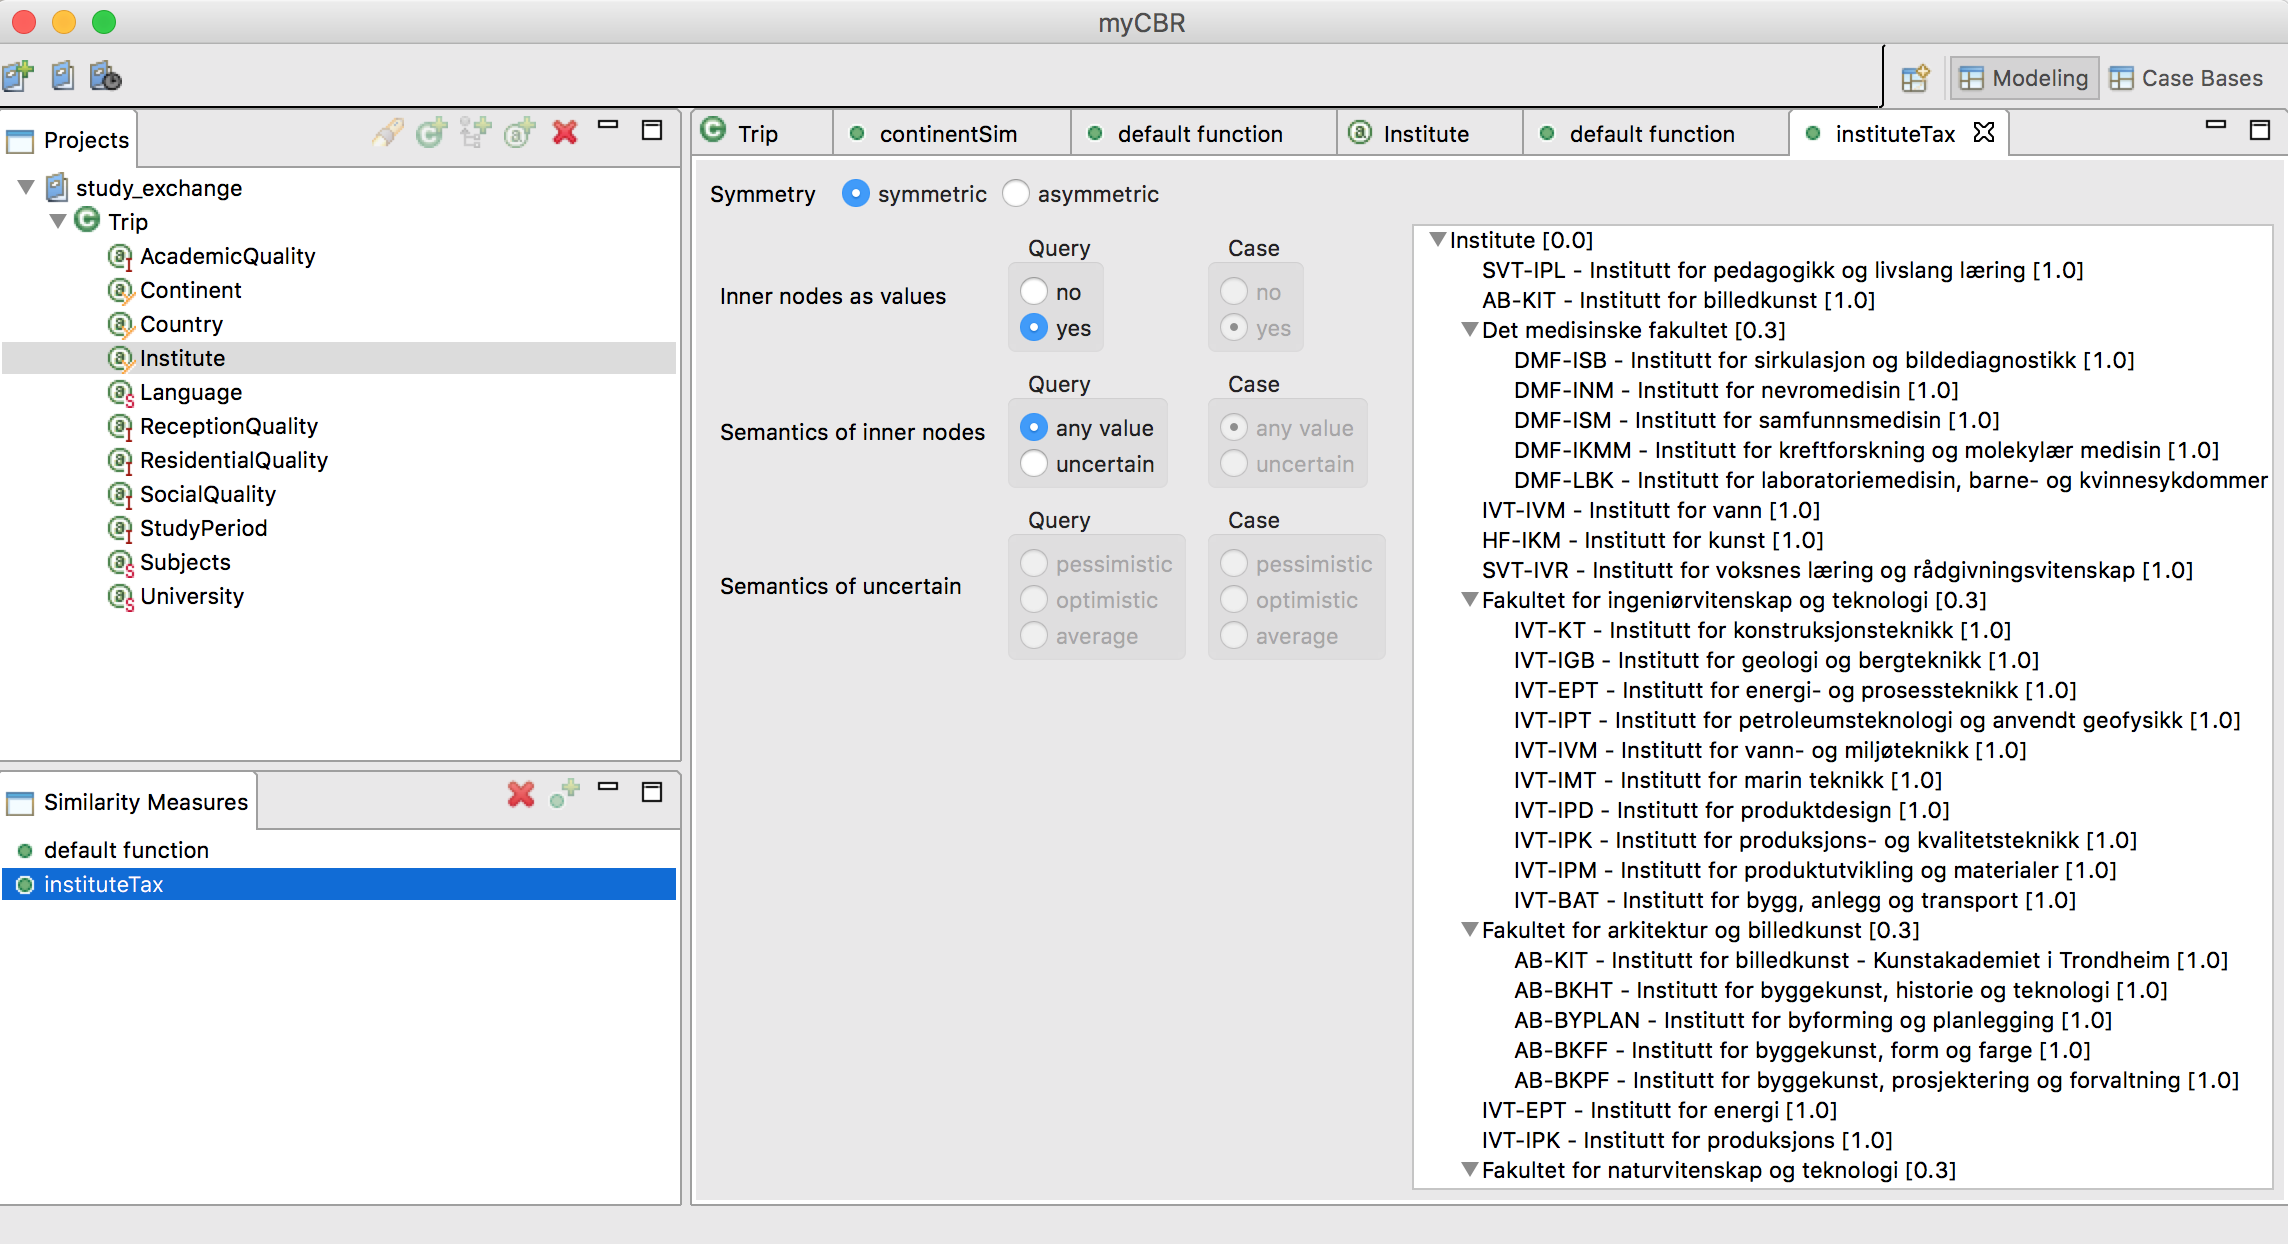
\includegraphics[width=8cm]{fig/myCBRworkbench.png}
    \caption{Example of modelling the taxonomy function from myCBR workbench}
\end{figure}



\section{Case-based Recommender Systems}\label{sec:case_based_recommender_systems}
Recommender systems are used extensively in both research and commercial products. These systems provide several possible solutions that might be viable for the user to choose. Several published research papers have explored different approaches to recommender systems\cite{mulyana2015case}\cite{quijano2011happy}.

Case-based reccommender systems use CBR as the underlying technique but has some differences compared to other implementations of CBR. The main differences being:
 
\begin{itemize}
    \item Less direct feedback and adaption
    \item More than one solution (recommendation) might be viable
\end{itemize}

There are mainly two types information a recommendation can be based on. The first being collaborative filtering which uses the rating and opinions of other user who has experienced the product or gone through the same process. The second being content based filtering which is based on the descriptions and information about the content, i.e static information like features, price, functionality and requirements. 



\section{Software Usability}




\cleardoublepage